\chapter{Extracci� de refer�ncies}
\label{chapter:refextraction}

Un cop hem aconseguit trobar p�gines que contenen informaci� de l'article pel qual volem generar la refer�ncia bibliogr�fica, �s moment d'extreure aquesta informaci� i formatar-la. En aquest cap�tol tractarem dels problemes que hem trobat a l'hora d'extreure la in

\section{\textit{Wrappers}}
En el nostre context, anomenarem \textit{wrapper} a una classe que implementa una s�rie de m�todes establerts i que, a partir d'un text o document d'entrada, permet extreure'n certa informaci�. Podem imaginar-ho com un filtre que nom�s ens deixa veure una part del document que ens interessa.
\begin{figure}[h!]
\begin{center}
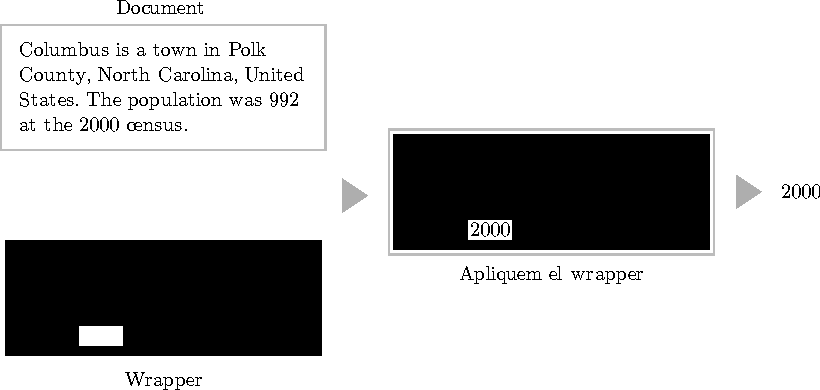
\includegraphics[scale=0.8]{figures/wrapper_sample.pdf}
\caption{Exemple de la funci� d'un \textit{wrapper}}
\label{fig:wrapper-desc}
\end{center}
\end{figure}

A la nostra aplicaci� tindrem els dos tipus de \textit{wrapper} que es descriuen a continuaci�.

\subsection{\textit{Field Wrappers}}
Es tracta de \textit{wrappers} que s'encarreguen d'extreure �nicament un dels camps de la refer�ncia a la vegada. 

En un principi vam comen�ar a implementar aquests \textit{wrappers} manualment, per� aix� comporta diversos problemes:
Aquests 

\subsection{\textit{Reference Wrappers}}
Aquest tipus de \textit{wrappers} extreuen el text corresponent a una refer�ncia sencera. El gran avantatge que tenen �s que habitualment permeten extreure molta m�s informaci� i amb una confian�a molt m�s gran.  Ara per ara, el sistema nom�s suporta refer�ncies \BibTeX{}, per� es podria ampliar amb qualsevol altre format.

\paragraph{}
El problema, �s que normalment no es troben a la mateixa p�gina retornada pels cercadors, sin� que cal seguir algun enlla�. A m�s, hi ha moltes biblioteques digitals que no ofereixen les refer�ncies en \BibTeX{} sin� en altres formats com ara \textit{RIS}, \textit{MODS}, etc.



Aquests \textit{wrappers} s'han implementat manualment.



\section{Validaci� de refer�ncies}
\subsubsection{\textit{Parsing} de refer�ncies}
Per poder validar les refer�ncies obtingudes a partir dels \textit{reference wrappers}, �s necessari analitzar-les sint�cticament per tal de poder validar cadascun dels camps. Per aquest motiu, l'aplicaci� disposa d'un \textit{parser} de refer�ncies en format \BibTeX{}.


\section{Format de refer�ncies}

Com a detalls de la implementaci�, nom�s comentar que tindrem un jerarquia de classes anomenades \textit{generadors}; que 